%! alt Acute triangle ABC inscribed in a circle with centre O and radius 13, with BC = 24. M is the midpoint of the arc BC not containing A, and the bisector AM passes through the incentre I. The highlighted circle with centre M passes through B, I and C, and MB = MI = MC.
%! after_paragraph 1
%! scale 1/8
% The shared preamble of every Cevian figure. pipeline/figures turns these colours into theme-aware paint,
% and refuses any other colour, so draw only with them:
%   figink (lines and labels), figaux (construction lines), figaccent (the object the argument turns on),
%   figtint and figaccenttint (light fills).
\documentclass[border=1.5pt]{standalone}
\usepackage{tkz-euclide}
\definecolor{figink}{RGB}{0,0,0}
\definecolor{figaux}{RGB}{85,85,85}
\definecolor{figaccent}{RGB}{192,57,43}
\definecolor{figtint}{RGB}{221,221,221}
\definecolor{figaccenttint}{RGB}{245,213,208}
% tkz-euclide's defaults draw circles, compasses and marks in 50% grey and fill points with a tint.
\makeatletter
\def\tkz@otherlinecolor{figink}
\def\tkz@euc@circlecolor{figink}
\def\tkz@euc@compasscolor{figink}
\def\tkz@euc@mkcolor{figink}
\def\tkz@mk@fill{figink}
\def\tkz@euc@pointfillcolor{figink}
\makeatother
\tkzSetUpLine[color=figink,line width=.7pt]
\tkzSetUpArc[color=figink,line width=.7pt]
\tkzSetUpCompass[color=figink,line width=.5pt]
\tkzSetUpPoint[color=figink,fill=figink,size=3.1pt]
\tikzset{
  every picture/.style={line cap=round,line join=round,color=figink},
  circle style/.append style={color=figink,line width=.7pt},
  aux/.style={color=figaux,line width=.45pt,dash pattern=on 2.6pt off 2pt},
  key/.style={color=figaccent,line width=1pt},
  mk/.style={color=figink,line width=.5pt},
  lbl/.style={color=figink,inner sep=2.2pt},
  len/.style={color=figink,inner sep=1.5pt,font=\small},
}

\begin{document}
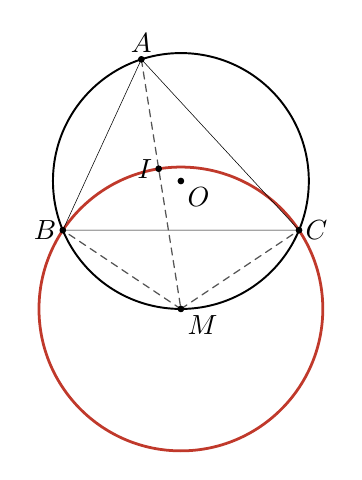
\begin{tikzpicture}
\tkzDefPoint(0.0,0.0){O} %! O = (0, 0)
\tkzDefPoint(-1.5000000,-0.62500000){B} %! B = (-12, -5)
\tkzDefPoint(1.5000000,-0.62500000){C} %! C = (12, -5)
\tkzDefPoint(-0.50215262,1.5454668){A} %! A = polar(O, 13, 108)
\tkzDefPoint(0.0,-1.6250000){M} %! M = (0, -13)
\tkzDefPoint(-0.28201624,0.15558048){I} %! I = incentre(A, B, C)
%! fact dist(B, C) == 24
%! fact on_circle(A, O, 13)
%! fact on_circle(B, O, 13)
%! fact on_circle(M, O, 13)
%! fact collinear(I, A, M)
%! fact equal(dist(M, I), dist(M, B))
%! fact equal(dist(M, C), dist(M, B))
%! fact dist(M, B)**2 == 208
\tkzDrawCircle(O,A)
\tkzDrawCircle[key](M,B)
\tkzDrawPolygon(A,B,C)
\tkzDrawSegment[aux](A,M)
\tkzDrawSegments[aux](M,B M,C)
\tkzDrawPoints(A,B,C,O,M,I)
\tkzLabelPoint[above,lbl](A){$A$}
\tkzLabelPoint[left,lbl](B){$B$}
\tkzLabelPoint[right,lbl](C){$C$}
\tkzLabelPoint[below right,lbl](O){$O$}
\tkzLabelPoint[below right,lbl](M){$M$}
\tkzLabelPoint[left,lbl](I){$I$}
\end{tikzpicture}
\end{document}
